
\documentclass[oneside]{book}
\usepackage{book}
\title{Jaseci and Jac}
\author{Jason Mars}


\newcommand{\printfigGraphTypes}{
    \begin{figure}
        \begin{subfigure}{.5\textwidth}
            \centering
            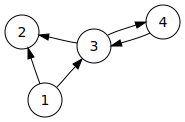
\includegraphics[width=.8\linewidth]{assets/images/Directed_graph_no_background.svg.pdf}
            \caption{Directed graph with cycle between nodes three and four.}
            \label{fig:directedgraph}
        \end{subfigure}
        \begin{subfigure}{.5\textwidth}
            \centering
            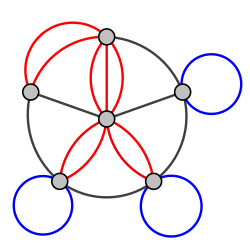
\includegraphics[width=.8\linewidth]{assets/images/Multi-pseudograph.svg.pdf}
            \caption{Multigraph with parallel edges and self-loops}
            \label{fig:multigraph}
        \end{subfigure}%
        \caption[]{Examples of first order graph symantics supported by Jaseci.\footnotemark}
        \label{fig:graph_examples}
    \end{figure}
    \footnotetext{Images credits to wiki contributers~\cite{wiki:Directed_graph_no_background.svg,wiki:Multi-pseudograph.svg}}
}


\newcommand{\printfigHelloWorldBaby}{
    \begin{figure}%{r}{0.5\textwidth}
        \centering
        \includegraphics[width=.3\linewidth]{assets/images/hello_world_baby.jpg}
        \caption[]{World's youngest coder with valid HTML on shirt.\footnotemark}
        \label{fig:hello_baby}
    \end{figure}
    \footnotetext{Image credit to wiki contributer~\cite{wiki:hello_world_baby.jpg}}
}
\newglossaryentry{christen}
{
    name=christen,
    description={to name or dedicate (something, such as a piece of code) by a ceremony that often involves breaking a bottle of champagne}
}
\newglossaryentry{pwn}
{
    name=pwn,
    description={the act of dominating a person, place, or thing. (...or a piece of code)}
}

\newglossaryentry{gobbledygook}
{
    name=gobbledygook,
    description={language that is meaningless or is made unintelligible by excessive use of abstruse technical terms; nonsense}
}
\newglossaryentry{bleh}
{
    name=bleh,
    description={mildly yucky}
}
\newglossaryentry{leet}
{
    name=leet,
    description={v. hyper-sophisticated from a coding perspective, n. a language used by \gls{leet} \gls{haxor}s}
}

\newglossaryentry{haxor}
{
    name=haxor,
    description={\gls{leet} spelling of hacker}
}
\newglossaryentry{coder}
{
    name=coder,
    description={the superior human}
}
\newglossaryentry{Jaseci jolt}
{
    name=Jaseci jolt,
    description={an insight derived from Jaseci that serves as a high voltage bolt of energy to the mind of a sharp coder.}
}
\newglossaryentry{common languages}
{
    name=common languages,
    description={typical languages programmers use to write commercial software, (e.g., C, C++, Java, Javascript, Python, Ruby, Go, Perl, PHP, etc.)}
}

\newglossaryentry{grok}
{
    name=grok,
    description={to fully comprehend and understand deeply }
}

\newglossaryentry{sick}
{
    name=sick,
    description={\gls{redonkulous}}
}

\newglossaryentry{redonkulous}
{
    name=redonkulous,
    description={\gls{dope}}
}

\newglossaryentry{dope}
{
    name=dope,
    description={\gls{sick}}
}

\newglossaryentry{goo goo gaa gaa}
{
    name=goo goo gaa gaa,
    description={the language of babies}
}

\newglossaryentry{directed graphs}
{
    type=technical,
    name=directed graphs,
    description={a directed graph (or digraph) is a graph that is made up of a set of vertices connected by directed edges (think edges as arrows as opposed to lines) often called arcs}
}
\newglossaryentry{undirected graphs}
{
    type=technical,
    name=undirected graphs,
    description={a graph made up of vertices (also called nodes or points) which are connected symmetrically by edges (also called links or lines)}
}

\newglossaryentry{multigraphs}
{
    type=technical,
    name=multigraph,
    description={a graph which is permitted to have multiple edges (also called parallel edges[1]), that is, edges that have the same end nodes}
}

\newglossaryentry{hypergraphs}
{
    type=technical,
    name=hypergraph,
    description={a hypergraph is a generalization of a graph in which an edge can join any number of vertices in contrast to connecting exactly two vertices}
}

\newglossaryentry{contexts}
{
    type=technical,
    name=contexts,
    description={A set of key value pairings that serve as a data payload attributable to nodes and edges in Jaseci graphs}
}

\newglossaryentry{walker}
{
    type=technical,
    name=walker,
    description={An abstraction in the Jaseci machine and Jac programming language that represents a computational agent that computes and travels along nodes and edges of a graph}
}

\newglossaryentry{sentinel}
{
    type=technical,
    name=sentinel,
    description={Overseer of walkers and architype nodes and edges.}
}
\newglossaryentry{IMHO}
{
    name=IMHO,
    description={Acronym for ``In My Humble Opinion''}
}

\newglossaryentry{WSL}
{
    type=technical,
    name=WSL,
    description={Windows Subsystem for Linux}
}
\newglossaryentry{dynamically typed language}
{
    type=technical,
    name=dynamically typed language,
    description={a language is dynamically typed if the type is associated with run-time values, and not named variables/fields/etc. This means that a programmer can code a bit quicker not having to specify types statically.}
}

\begin{document}


\def\JJ{JASECI \& JAC} % Title
\def\BB{BIBLE} % Title
\title{\JJ \BB}

\def\Me{Jason Mars} % Author
\author\Me

\def\VER{v1.0}
\definecolor{title_white}{rgb}{1,1,1}
\definecolor{title_grey}{rgb}{0.6,0.6,0.6}


\newpagecolor{black}
\vspace{\fill}
\addtolength{\topmargin}{1in}



\setstretch{10.0}


\begingroup
\bf\centering
{\color{title_white} \scalebox{4}[4]{\JJ}}\\
{\color{title_grey} \scalebox{7}[7]{\BB}}\\
{\color{title_white} \scalebox{2}[2]{\Me}}\par
{\color{title_white} \scalebox{2}[2]{\VER}}
\endgroup


\pagebreak
\restorepagecolor
\thispagestyle{empty}
%After title we restore all margins. 
\newgeometry{margin=1in}
\setstretch{1.0}



\newpagecolor{black}
\vspace{\fill}
\addtolength{\topmargin}{1.5in}



\setstretch{2.0}


\begingroup
\bf\centering
\color{white}\LARGE
Warning: This book may trigger you.
\vspace{1in}
\par \Large \setstretch{1.0}
If after reading that sentence you feel a sense of concern, this book WILL trigger you and you'll need to refer to the previous page and continue. If you are not concerned after reading the warning, continue with caution.

\endgroup


\pagebreak
\restorepagecolor

%After title we restore all margins. 
\newgeometry{margin=1in}
\setstretch{1.0}

\normalem
\cleardoublepage % Make toc appear on right side.
\setcounter{secnumdepth}{3} % toc is 2 level deep.
\tableofcontents
\pagebreak
\printglossary[title=Terms Used, toctitle=List of Terms]
\printglossary[type=technical, title=Technical Terms Used, toctitle=List of Technical Terms]


\chapter*{Preface}
\addcontentsline{toc}{chapter}{Preface}

The way we design and write software to do computation and AI today sucks. It's a vat of boiling poop, mixed with pee, slowly swirling and bubbling toward that dehydrated semi-solid state of goop that serves to repel and repulse most normal people only attracting the few unfortunate-fortunate folks that happen to be obsessed with \gls{scat}.
\par
Hrm, too much? Probably. I guess you'd expect me to use concrete examples and cite evidence to make my points, me being a professor and all. I mean, I could write something like \textit{``The fundamental imperative programming model utilized in near all of the production software produced in the last four decades has not changed since blah blah blah..."} to meet expections. I'd certainly sound more credible and perhaps super smart. Well, I'm not going to do that here. Let's have fun. Afterall, Jaseci has never been work for me, its play. Very ambitious play granted, but play at it's core.
\par
Everything here is based on my opinion and intution. That suffices for me, and I hope it does for you. I have spent many decades coding and leading teams who code, but its my gut that tells me that we can do better. This book describes my attempt at better. I hope you find value in it. If you do, awesome! If you don't, also awesome.

\chapter{Introduction}
There has been a fundamental paradigm shift in the landscape of how we build software over the last 2 decades.
The compute stack was originally envisaged with the assumption that a single program would run on a single machine.
In this traditional model, system software abstractions subsumed the management of processor, memory, disk and physically connected peripherals within the context of the machine.
However, this landscape rapidly changed with the evolution toward software being served on the backbone provided by the internet.
Now, an `application' is realized through the cooperation of multiple distinct sub-applications (services) running collaboratively.
For example a single application my contain self one or more self-contained database, memcache, logging, application logic, AI model applications interfacing each other over APIs as shown in Figure~\ref{fig:intro} (left).
We call these applications \emph{diffuse applications}.


This work contends that the fundamental programming paradigms in computing has not evolved at pace.
The abstractions envisioned during the era of the single machine computational model is still present at the programming interface and throughout the runtime stack leading to significant and costly complexity.


To address this complexity, two keystone abstractions have recently emerged to facilitate the development of these diffuse applications.
The first of these abstractions is the introduction and rapid dissemination of containerization service platforms.
With what started as a key insight articulated in ``The Datacenter as a Computer,'' Google would innovate their Borg system and ultimately released it open source as Kubernetes.
With Kubernetes, the underlying hardware resources would be abstracted away with the introduction of \emph{pods} (virtual machines), and other resources that can be virtually networked together and otherwise configured irrespective of the physical hardware.
Today, Kubernetes is the most prevalent containerized service abstraction layer in cloud computing.
The second of keystone abstraction would be coined ``Severless Computing'' and gained prominence with the introduction of Amazons Lamda functions.
This FaaS abstraction would facilitate the development of diffuse applications at the level of functions and abstract away the underlying containerized service ecosystem.
A programer can simply make function calls in their favorite language without every needing to be aware of where the function will run nor the system level resources that would be allocated or managed.

\begin{figure}[tb]
    \centering
    \includegraphics[width=\linewidth]{figures/jaseci_stack.pdf}
    \caption{Comparison between status quo development of production grade \emph{diffuse} applications (left), and the Jaseci technology stack that hides and automates an expanded set of subsystems through raising the level of abstraction (right).}
    \label{fig:intro}
\end{figure}



Though these two abstractions have been highly impactful, these innovations in our stack architecture represent a bottom up evolution of abstractions.
As a result, programmers are still left with single-machine abstractions at the programming interface and must grapple with a significant amount of complexity.
For example, traditional languages and their runtime stacks are predominately designed with the goal of hiding and managing intra-machine resources while what is needed for diffuse applications is the hiding and management of inter-machine resources.
Analogous to the virtualization and management of allocated memory on the heap provided by garbage collectors in modern languages (intra-machine), the virtualization and management of resources such as microservice creation, scheduling and orchestration alongside policies for organizing distributed databases, mem caches, logging and other highly complex subsystems (inter-machine) is not only needed, but as we show in this work, possible and practical.
Without this raising of the level of abstraction, it has become prohibitively difficult for a single engineer to invent, build, deploy, launch, and scale modern cutting edge applications.

To the best of our knowledge, we are not aware of a thorough, wholistic, and top-down design of a serverless programming paradigm and computational stack from the language level down through the system runtime stack to hide this expanded set of resources.

In this work, we present a wholistic design approach with the goal of abstracting away and automating a new class of underlying systems, allowing a programmer to articulate solutions and diffuse applications at the problem level.
We present the design of a \emph{diffuse runtime execution engine} we call \textbf{Jaseci}, and a \emph{data-spacial programming language} we call \textbf{Jac}.

The design of Jaseci and Jac has initially been inspired to by sophisticated emerging AI applications at scale and is driven by two key insightss.

\begin{itemize}

    \item \emph{Higher level abstractions are needed at the language level to allow single creators to work at the problem level to build end-to-end diffuse AI products.}
    \item \emph{A new set of abstractions across the language runtime and system stack is needed to automate and hide the class of inter-machine resources from the programmer.}

\end{itemize}

\noindent
To this end we present techniques across two categories,

\begin{enumerate}


    \item \emph{Jac Language} - A language that introduces a new set of abstractions, namely \textbf{data-spacial scoping} and \textbf{agent oriented programming}. These abstractions natively facilitates the emerging need to reason about and solve problems with graph representations as well as the need for algorithmic modularity and encapsulation to hide a new class of inter-machine resources.
    \item \emph{Jaseci Diffuse Runtime Engine} - A runtime that raises the abstraction layer to the problem solving level where the runtime engine subsumes responsibility for not only for the optimization of program code, but the orchestration, configuration, and optimization of the full cloud compute stack and inter-machine resources (such tasks as container formation, scaling and optimization).


\end{enumerate}


Jaseci and Jac is fully functional, open-source~\cite{jaseci-website,jaseci-github,jaseci-pypi}, and used in production for four real-world products today.
These commercial products were built entirely on the Jaseci staci and includes Myca~\cite{myca-website}, HomeLendingPal~\cite{hlp-website},  ZeroShotBot~\cite{zsb-website} and TrueSelph~\cite{ts-website}.
Across these and other projects, the Jac language has been used by dozens of programmers in the creation of production software and Jaseci deployments support tens of thousands of production queries per day currently.
In practice, our initial infrastructure has been leveraged in practice to achieve 10x reduction in development time and near 100\% elimination of typical backend code needed for a complicated AI based application.

The specific contributions of this paper include:
\begin{itemize}
    \item We formulate the problem of development complexity and present a top down programing paradigm and runtime stack for diffuse applications.
    \item We describe the design and implementation Jaseci's \textbf{diffuse runtime execution engine}.
    \item We introduce Jac, a language that implements a \textbf{data-spacial} programming paradigm (the first of its kind).
    \item We describe the utility of Jaseci and Jac through real world case studies of building out a real production scale-out product.
\end{itemize}

We find that the wholistic design philosophy and resulting paradigm of Jaseci and Jac is a promising one.
Multiple development teams have adopted the data spacial programming model of Jac and the diffuse runtime execution engine in Jaseci to build sophisticated AI products with significantly reduced complexity and teaming.




\part{World of Jaseci}
\label{part:jsword}
\chapter{What and Why is Jaseci?}
\section{Viewing the Problem Landscape Spacially}
\section{Compute via The Collective, Ants in the Colony}

\chapter{Abstrations of Jaseci}
\minitoc
\section{Graphs, the Friend that Never Gets Invited to the Party}
There's something quite strange that has happend with our \gls{common languages} over the years, ...decades. When you look at it, almost every data structure we programmers use to solve problems can be modeled formally as a graph, or a special case of a graph, (save perhaps hash tables). Think about it, stacks, lists, queues, trees, heaps, and yes, even graphs, can be modeled with graphs. But, low and behold, no common language ustilizes the formal semantics of a graph as its first order abstraction for data or memory. I mean, isn't it a bit odd that practically every data structure covered in the language-agnostic classic foundational work \textit{Introduction to Algorithms}~\cite{intro_to_algo} can most naturally be be reasoned about as a graph, yet none of the common languages have built in and be designed around this primitive. I submit that the graph semantic is insanely rich, very nice for us humans to reason about, and, most importantly for the purpose of Jaseci, is inherently well suited for the conceptualization and reasoning about computational problems, especially AI problems.
\par
There are a few arguments that may pop into mind at this point of my conjecture.
\begin{itemize}
    \item ``Well there are graph libraries in my favorite language that implement graph symantics, why would I need a language to force the concept upon me?''
          or
    \item ``Duh! Interacting with all data and memory through graphical abstractions will make the language ssllooowww as hell since memory in hardware is essitially a big array, what is this dude talking about!?!?''
\end{itemize}
\par
For the former of these two challenges, I counter with two points. First, the core design languages are always based upon their inherent abstractions. With graphs not being one such abstraction, the language's design will not be optimized to empower programmers to nimbly do gymnastics with rich language symantics that correspond to the rich semantics graphs offer (You'll see what I mean in later chapters).
\par
For the latter question, I'd respond, ``Have you SEEN the kind of abstractions in modern languages!?!? It's rediculous, lets look at python dictionaries, actually scratch that, lets keep it simple and look at dynamic typing in general. The runtime complexity to support dynamic typing is most certainly higher than what would be needed to support graph symantics. Duh right back at'ya!''
\subsection{Yes, But What Kind of Graphs}

There are many categories of graphs to consider when thinking about the abstractions to support in Jaseci. There are rules to be defined as to the availabe semantics of the graphs. Should all graphs be \gls{directed graphs}, should we allow the creation of \gls{undirected graphs}, what about parallel edges or \gls{multigraphs}, are those explicitly expressible or discouraged / banned, can we express \gls{hypergraphs}, and what combination of these graphical sematics should be able to be manifested and manipulated through the programming model. At this point I can feel your eyes getting droopy and your mind moving into that intermediary state between concious and sleeping, so let me cut to the answer.
\par
\printfigGraphTypes
In Jaseci, we elect to assume the following semantics:
\begin{enumerate}
    \item Graphs are directed (as per Figure~\ref{fig:directedgraph}) with a special case of a doubly directed edge type which can be utilized practically as an undirected edge (imagine fusing the two edges between nodes 3 and 4 in the figure).
    \item Both nodes and edges have their own distinct identities (i,e. an edge isn't representable as a pairing of two nodes). This point is important as both nodes and edges can have \gls{contexts}.
    \item Multigraphs (i.e., parallel edges) are allowed, including self-loop edges (as per Figure~\ref{fig:multigraph}).
    \item Graphs are not required to be acyclic.
    \item No hypergraphs, as I wouldn't want Jaseci programmers heads to explode.

\end{enumerate}
\emph{As an aside, I would describe Jaseci graphs as strictly unstrict directed multigraphs that leverages the semantics of parallel edges to create a laymans `undirected edge' by shorthanding two directed edges pointed in opposite directions between the same two nodes.}
\par
\begin{nerd}
    I'd formally describe a Jaseci Graph as an $7$-tuple $(N,E,C,s,t,c_N,c_E)$, where
    \begin{enumerate}
        \item $N$ is the set of nodes in a graph
        \item $E$ is the set of edges in a graph
        \item $C$ is the set of all contexts
        \item $s$: $E \rightarrow V$, maps the source node to an edge
        \item $t$: $E \rightarrow V$,  maps the target node to an edge
        \item $c_N$: $N \rightarrow C$, maps nodes to contexts
        \item $c_E$: $E \rightarrow C$, maps edges to contexts
    \end{enumerate}
    An undriected edge can then be formed with a pair of edges $(x, y)$ if three conditions are met,
    \begin{enumerate}
        \item $x, y \in E$
        \item $s(x) = t(y)$, and $s(y) = t(x)$
        \item $c_E(x) = c_E(y)$
    \end{enumerate}
\end{nerd}
\par
If you happend to have read that formal definition and didn't enter deep comatose you may be wondering ``Whoa, what was that context stuff that came outta nowhere! What's this guy trying to do here, sneaking a new concept in as if it was already introduced and described.''
\par
Worry not friend, lets discuss.
\subsection{Putting it All Into Context}

A key principle of Jaseci is to reshape and reimagine how we view data and memory. We do so by fusing the concept of data with the intuitive and rich semantics of graphs as the lowest level primitive to view memory.

\begin{nerd}
    A context is a representation of data that can be expressed simply as a $3$-tuple $(\sum_K,\sum_V,p_K)$, where
    \begin{enumerate}
        \item $\sum_K$ is a finite alphabet of keys
        \item $\sum_V$ is a finite alphabet of values
        \item $p_K$ is the pairing of keys to values
    \end{enumerate}
\end{nerd}
\section{Walkers}
One of the most important abstractions introduced in Jaseci is that of the \texttt{walker}.
The semantics of this abstraction is unlike any that has existed in any programming language before.

In a nutshell, a walker is a unit of execution that retains state (its local scope) as it travels over a graphs.
Walkers `walk' from node to node in the graph and executing its body.

The walker's body is specified with an opening and closing braces (\texttt{ \{ \} }) and is executed to completion on each node it lands on.
In this sense a walker iterates while spooling through a sequence of nodes that it `takes' using the \lstinline{take} keyword.
We call each of these iterations \emph{node-bound iterations}.

Variables declared in a walker's body takes two forms: its \emph{context variables}, those that retain state as it travels from node to node in a graph, and its \emph{local variables}, those that are reinitialized for each node-bound iterations.

Walkers present a new way of thinking about programmatic execution distinct from the near-ubiquitous function based asbtraction in other languages.
Instead of a functions scope being temporally pushed onto an ever increasing stack as functions call other functions.
Scopes can be spacially laid out on a graph and walkers can hop around the graph taking its scope with it.
A key difference in this model is in its introduction of data spacial problem solving.
In the former function-based model scopes become unaccessible upon the sub-call of a function until that function returns.
In contrast, walkers can access any scope at any time in a modular way.

When solving problems with walkers, a developer can think of that walker as a little self-contained robot or agent that can retain context as it spacially moves about a graph, interacting with the context in nodes and edges of that graph.

In addition to the introduction of the \lstinline{take} command to support new types of control flow for node-bound iterations. The keywords and semantics of \lstinline{disengage}, \lstinline{skip}, and \lstinline{ignore} are also introduced. These instruct walkers to stop walking the graph, skip over a node for execution, and ignore certain paths of the graph.
These semantics are describe in more detail later in the book.

[Entrypoints to a jac program, init recognized as default]

\section{Abilities}

Nodes, edges, and walkers can have \texttt{abilities}.
The body of an ability is specified with an opening and closing braces (\texttt{ \{ \} }) within the specification of a node, edge, or walker and specify a unit of execution.

Abilities are most closely analogous to methods in a traditional object oriented program, however they do not have the same semantics of a traditional function.
An ability can only interact within the scope of context and local variables of the node/edge/walker for which it is affixed and do not have a \texttt{return} semantic. (Though it is important to note, that abilities can always access the scope of the executing walker using the \lstinline{visitor} special variable as described below)

When using abilities, a developer can think of these as self-contained in-memory/in-data compute operations.

\section{\texttt{here} and \texttt{visitor}}

At every execution point in a Jac/Jaseci program there are two scopes visible, that of the walker, and that of the node it is executing on.
These contexts can be referenced with the special variables \lstinline{here} and \lstinline{visitor} respectively.
Walkers use \lstinline{here} to refer to the context of the node it is currently executing on, and abilities can use \lstinline{visitor} to refer to the context of the current walker executing.

\section{Actions}

Actions enables bindings to functionality specified outside of Jac/Jaseci and behave as function calls with returns.
These are analogous to library calls in traditional languages.
This external functionality in practice takes the form of direct binding to python implementations that are packaged up as a Jaseci action library.

\begin{nerd}
    Note: This action interface is the abstraction that allows Jaseci to do it's fancy inter-machine optimizations, auto-scaling, auto-componentization etc.
\end{nerd}

\chapter{Architecture of Jaseci and Jac}
\section{Anatomy of a Jaseci Application}
\section{The Jaseci Machine}
\subsection{Machine Core}
\subsection{Jaseci Cloud Server}

\chapter{Interfacing a Jaseci Machine}
\jacdot{dia_api_server_client}{.5}{Jaseci Interface Architecture}
Now that we know what Jaseci is all about, next lets roll up our sleeves and jump in. One of the best ways to jump into Jaseci world is to gather some sample Jac programs and start tinkering with them.
\par
Before we jump right into it, it's important to have a bit of an understanding of the the way the interface itself is architected from in the implementation of the Jaseci stack. Jaseci has a module that serves as its  the core interface (summarized in Table~\ref{tab:jsAPI}) to the Jaseci machine. This interface is expressed as a set of method functions within a python class in Jaseci  called \texttt{master}. (By the way, don't worry, it's ok to use ``master'', its not racialist, see Rant~\ref{rant:racistmaster} for more context). The `client' expressions of that interface in the forms of a command line tool \texttt{jsctl} and a server-side REST API built using Django~\footnote{Django ~\cite{django} is a Python web framework for rapid development and clean, pragmatic design}. Figure~\ref{dot:dia_api_server_client} illustrates this architecture representing the relationship between core APIs and client side expressions.
\printtabJSAPI
If I may say so myself the code architecture of interface generation from function signatures is elegant, sexy, and takes advantage of the best python has to offer in terms of its support for introspection. With this approach, as the set of functions and their semantics change in the \texttt{master} API class, both the JSCTL Cli tool and the REST Server-side API changes. We dig into this and tons more in the Part~\ref{part:crafting}, so we'll leave the discussion on implementation architecture there for the moment. Lets jump right into how we get started playing with some \gls{leet} Jaseci \gls{haxor}ing. First we start with JSCTL then dive into the REST API.


\section{JSCTL: The Jaseci Command Line Interface}
JSCTL or \texttt{jsctl} is a command line tool that provides full access to Jaseci. This tool is installed alongside the installation of the Jaseci Core package and should be accessible from the command line from anywhere. Let's say you've just checked out the Jaseci repo and you're in head folder. You should be able to execute the following.
\par
\shellout{jsctl_setup.shell}
\par
Here we've installed the Jaseci python package that can be imported into any python project with a directive such as \texttt{import jaseci}, and at the same time, we've installed the \texttt{jsctl} command line tool into our OS environment. At this point we can issue a call to say \texttt{jsctl --help} for any working directory.
\begin{nerd}
    Python Code~\ref{py:setup.py} shows the implementation of \texttt{setup.py} that is responsible for deploying the jsctl tool upon \texttt{pip3} installation of Jaseci Core.
    \pycode{setup.py}{setup.py for Jaseci Core}
\end{nerd}

\subsection{The Very Basics: CLI vs Shell-mode, and Session Files }
This command line tool provides full access to the Jaseci core APIs via the command line, or a shell mode. In shell mode, all of the same Jaseci API functionally is available within a single session. To invoke shell-mode, simply execute \texttt{jsctl} without any commands and jsctl will enter shell mode as per the example below.
\par
\shellout{jsctl_shell_mode.shell}
\par
Here we launched \texttt{jsctl} directly into shell mode for a single session and we can issue various calls to the Jaseci API for that session. In this example we issue a single call to \texttt{graph create}, which creates a graph within the Jaseci session with a single root node, then exit the shell with \texttt{exit}.
\par
The exact behavior can be achieved without ever entering the shell directly from the command line as shown below.
\par
\shellout{jsctl_cli_mode.shell}
\par
All such calls to Jaseci's API (summarized in Table~\ref{tab:jsAPI}) can be issued either through shell-mode and CLI mode.
\paragraph{Session Files}
At this point, it's important to understand how sessions work. In a nutshell, a session captures the complete state of a jaseci machine. This state includes the status of memory, graphs, walkers, configurations, etc. The complete state of a Jaseci machine can be captured in a \texttt{.session} file. Every time state changes for a given session via the \texttt{jsctl} tool the assigned session file is updated. If you've been following along so far, try this.
\par
\shellout{session_default.shell}
\par
Note from the first call to \texttt{ls} we have a session file that has been created call \texttt{js.session}. This is the default session file \texttt{jsctl} creates and utilizes when called either in cli mode or shell mode. After listing session files, notices the call to \texttt{graph list} which lists the root nodes of all graphs created within a Jaseci machine's state. Note \texttt{jsctl} lists two such graph root nodes. Indeed these nodes correspond to the ones we've just created when contrasting cli mode and shell mode above. Having these two graphs demonstrates that across both instantiations of \texttt{jsctl} the same session, \texttt{js.session}, is being used. Now try the following.
\par
\shellout{new_session.shell}
\par
Here we see that we can use the \texttt{-f} or \texttt{--filename} flag to specify the session file to use. In this case we list the graphs of the session corresponding to \texttt{mynew.session} and see the JSON representation of an empty list of objects. We then list session files and see that one was created for \texttt{mynew.session}. If we were to now type \texttt{jsctl --filename js.session graph list}, we would see a list of the two graph objects that we created earlier.
\paragraph{In-memory mode}
Its important to note that there is also an in-memory mode that can be created buy using the \texttt{-m} or \texttt{--mem-only} flags. This flag is particularly useful when you'd simply like to tinker around with a machine in shell-mode or you'd like to script some behavior to be executed in Jac and have no need to maintain machine state after completion. We will be using in memory session mode quite a bit, so you'll get a sense of its usage throughout this chapter. Next we actually see a workflow for tinkering.

\subsection{A Simple Workflow for Tinkering}

As you get to know Jaseci and Jac, you'll want to try things and tinker a bit. In this section, we'll get to know how \texttt{jsctl} can be used as the main platform for this play. A typical flow will involve jumping into shell-mode, writing some code, running that code to observe output, and in visualizing the state of the graph, and rendering that graph in dot to see it's visualization.
\paragraph{Install Graphvis}
Before we jump right in, let me strongly encourage you install Graphviz. Graphviz is open source graph visualization software package that includes a handy dandy command line tool call \texttt{dot}. Dot is also a standardized and open graph description language that is a key primitive of Graphviz. The \texttt{dot} tool in Graphviz takes dot code and renders it nicely. Graphviz is super easy to install. In Ubuntu simply type \texttt{sudo apt install graphviz}, or on mac type \texttt{brew install graphviz} and you're done! You should be able to call \texttt{dot} from the command line.
\par
Ok, lets start with a scenario. Say you'd like to write your first Jac program which will include some nodes, edges, and walkers and you'd like to print to standard output and see what the graph looks like after you run an interesting walker. Let role play.
\par
Lets hop into a \texttt{jsctl} shell.
\par
\shellout{wf_init.shell}
\par
Good, we're in! And we've set the session to be an in-memory session so no session file will be created or saved. For this play session we only care about the Jac program we write, which will be saved. The state of the Jaseci machine we run our toy program on doesn't really matter to us.
\par
Now that we've got our shell running, we first want to create a blank graph. Remember, all walkers, Jaseci's primary unit of computation, must run on a node. As default, we can use the root node of a freshly created graph, hence we need to create a base graph. But oh no! We're a bit rusty and have forgotten how create our initial graph using \texttt{jsctl}. Let's navigate the help menu to jog our memories.
\par
\shellout{wf_help_nav.shell}
\par
Ohhh yeah! That's it. After simply using \texttt{help} from the shell we were able to navigate to the relevant info for \texttt{graph create}. Let's use this newly gotten wisdom.
\par
\shellout{wf_graph.shell}
\par
Great! With this command a graph is created and a single root node is born. \texttt{jsctl} shares with us the details of this root graph node. In Jaseci, graphs are referenced by their root nodes and every graph has a single root node.
\par
Notice we've also set the \texttt{-set\_active} parameter to true. This parameter informs Jaseci to use the root node of this graph (in particular the UUID of this root node) as the default parameter to all future calls to Jaseci Core APIs that have a parameter specifying a graph or node to operate on. This global designation that this graph is the `active' graph is a convenience feature so we the user doesn't have to specify this parameter for future calls. Of course this can be overridden, more on that later.
\par
Next, lets write some Jac code for our little program. \texttt{jsctl} has a built in editor that is simple yet powerful. You can use either this built in editor, or your favorite editor to create the \texttt{.jac} file for our toy program. Let's use the built in editor.
\par
\shellout{wf_edit_jac.shell}
\par
The \texttt{edit} command invokes the built in editor. Though it's a terminal editor based on \texttt{ncurses}, you can basically use it much like you'd use any wysiwyg editor with features like standard cut \texttt{ctrl-c} and paste \texttt{ctrl-v}, mouse text selection, etc. It's based on the phenomenal pure python project from Google called \texttt{ci\_edit}. For more detailed help cheat sheet see Appendix~\ref{ci_help}. If you must use your own favorite editor, simply be sure that you save the fam.jac file in the same working directory from which you are running the Jaseci shell. Now type out the toy program in Jac Code~\ref{jac:fam.jac}.
\par
\jaccode{fam.jac}{Jac Family Toy Program}
\par
Don't worry if that looks like the most cryptic \gls{gobbledygook} you've ever seen in your life. As you learn the Jac language, all will become clear. For now, lets tinker around. Now save and quit the editor. If you are using the built in editor thats simply a \texttt{ctrl-s, ctrl-q} combo.
\par
Ok, now we should have a \texttt{fam.jac} file saved in our working directory. We can check from the shell!
\par

\par
Now, Lets create a sentinel for our Jac.
\par
\shellout{wf_sent_reg.shell}
\par
Next, we can look at some of the objects loaded into our Jaseci machine.
\par
\shellout{wf_aliases.shell}
\par
Now, lets run our walker on the root node of the graph we created.
\par
\shellout{wf_run_walker.shell}
\par
Finally, we can see what our graph looks like!!
\par
\shellout{wf_dot_render.shell}
\shellout{wf_dot_render_save.shell}
\par
Awesomeness! We are Jac \Gls{haxor}s now!

\section{Jaseci REST API}

\section{Full Spec of Jaseci Core APIs}
\subsection{config APIs}
\subsection{alias APIs}
\subsection{architype APIs}
\subsection{graph APIs}
\subsection{sentinel APIs}
\subsection{walker APIs}
\subsection{Miscellaneous APIs}

\part{The Jac Programming Language}
\label{part:jacd}
\input{assets/tex/jac/language_basics.tex}

\chapter{Graphs, Architypes, and Walkers in Jac}



%%%%%%%%%%%%%%%%%%%%%%%%%%%%%%
\section{Structure of a Jac Program}

\par [Introduce structure of a jac program] \par
\par [Specify the differnce between graph architypes, graph instantiations, and walkers]\par
\par [Present simple program that utilizes the structures]\par
\par [Present variations on articulating the same program]\par
\par [Code blocks]\par

\begin{nerd}
    Grammar~\ref{gram:jac.g4:3:16} shows the lines from the formal grammar for Jac that presents the high level structure of a Jac program.
    \gramcoderange{jac.g4}{Jac grammar clip relevant to arithmetic}{3}{16}
\end{nerd}

%%%%%%%%%%%%%%%%%%%%%%%%%%%%%%
\section{Graphs as First Class Citizens}

%%%%%%%
\par
\jaccode{jac_simple_walker.jac}{Simple walker creating and connected nodes}
\par
\jacdotnw{jac_simple_walker}{.3}{Graph in memory for JC~\ref{jac:jac_simple_walker.jac}}


%%%%%%%
\par
\jaccode{jac_named_node_edge.jac}{Creating named node types}
\par
\jacdotnw{jac_named_node_edge}{.3}{Graph in memory for JC~\ref{jac:jac_named_node_edge.jac}}

%%%%%%%
\par
\jaccode{jac_spawn_connect.jac}{Connecting nodes within spawn statement}
\par
\jacdotnw{jac_spawn_connect}{.3}{Graph in memory for JC~\ref{jac:jac_spawn_connect.jac}}

%%%%%%%
\par
\jaccode{jac_connect_chain.jac}{Chaining node connections using the connect operator}
\par
\jacdotnw{jac_connect_chain}{.3}{Graph in memory for JC~\ref{jac:jac_connect_chain.jac}}

%%%%%%%%%%%%%%%%%%%%%%%%%%%%%%
\section{Walkers as First Class Citizens}

%%%%%%%
\par
\jaccode{jac_walker_spawn_walker.jac}{Walkers spawning other walkers}
\par
\shellout{jac_walker_spawn_walker.jac.output}
\par
\jacdotnw{jac_walker_spawn_walker}{.3}{Graph in memory for JC~\ref{jac:jac_walker_spawn_walker.jac}}

%%%%%%%
\par
\jaccode{jac_walker_returns.jac}{Getting returned values from spawned walkers}
\par
\shellout{jac_walker_returns.jac.output}
\par
\jacdotnw{jac_walker_returns}{.3}{Graph in memory for JC~\ref{jac:jac_walker_returns.jac}}
\par
\jaccode{jac_walker_returns_alt.jac}{Increasing elegance by remembering spawns are expressions}

%%%%%%%
Walkers are entry points to all valid jac programs
\par


%%%%%%%%%%%%%%%%%%%%%%%%%%%%%%
\section{Architypes and Actions}

%%%%%%%
\par
\jaccode{jac_contexts.jac}{Binding member contexts to nodes and edges
}
\par
\shellout{jac_contexts.jac.output}
\par
\jacdotnw{jac_contexts}{.3}{Graph in memory for JC~\ref{jac:jac_contexts.jac}}

%%%%%%%
\par
\jaccode{jac_contexts_alt.jac}{Binding contexts with less code
}
\par
\shellout{jac_contexts_alt.jac.output}

%%%%%%%
\par
\jaccode{jac_copy_assign.jac}{Copy assigning from node to node
}
\par
\shellout{jac_copy_assign.jac.output}
\par
\jacdotnw{jac_copy_assign}{.5}{Graph in memory for JC~\ref{jac:jac_copy_assign.jac}}

%%%%%%%
\par
\jacdotnw{jac_action}{.3}{Graph in memory for JC~\ref{jac:jac_action.jac} and~\ref{jac:jac_node_action.jac}}
\par
\jaccode{jac_action.jac}{Basic action in walker
}
\par
\shellout{jac_action.jac.output}
\par
\jaccode{jac_node_action.jac}{Basic action in node
}

%%%%%%%
\par
\jaccode{jac_preset_action.jac}{Basic action with presets and event triggers
}
\par
\shellout{jac_preset_action.jac.output}
\par
\jaccode{jac_node_act_note.jac}{Basic action with presets and event triggers
}
\par [Only nodes can have with entry/exit`' and presets]
\par [can leave output (push returns) in node and walker]

%%%%%%%
\par
\jaccode{jac_local_action.jac}{Specifying your own actions
}
\par
\shellout{jac_preset_action.jac.output}
%%%%%%%
\par
\jaccode{jac_local_wlk_action.jac}{Walkers can have actions, and calling own actions
}
\par [here and visitor should be present everywhere]
\par [here should point to wherever the walker is on at all times]
\par [directly accessing variables in a nodes ability will not necesarily map to here]

\chapter{Walkers Navigating Graphs}



%%%%%%%%%%%%%%%%%%%%%%%%%%%%%%
\section{Taking Edges (and Nodes?)}

\subsection{Basic Walks}

%%%%%%%
\par
\jaccode{jac_take.jac}{Basic example of walker traveling graph
}

%%%%%%%
\par
\jaccode{jac_take_fanout.jac}{Fan out style takes
}

\subsection{Breadth First vs Depth First Walks}
\par
\jacdotnw{jac_walk_bfs}{.7}{Graph in memory for JC~\ref{jac:jac_walk_bfs.jac}}
If you've played with the basic \lstinline{take} command a bit you would notice that by default it results in a breadth first traversal of a graph.
However, the \lstinline{take} command is indeed quite flexible.
You can specify an orientation of the \lstinline{take} command to navigate with a breadth first or a depth first traversal.
\par
\jaccode{jac_walk_bfs.jac}{Breadth first navigation with take vs depth first}
\par
Take for example the program shown in JC~\ref{jac:jac_walk_bfs.jac}.
First we observe the definition of a static three level binary tree with the graph \lstinline{example} on line 3.
This is a vanilla structure as depicted in Figure~\ref{dot:jac_walk_bfs}.
Two walkers are present in this example, one walker \lstinline{walk\_with\_breadth}, for which we observe a call to \lstinline{take:bfs -->;} indicating a breadth first traversal, and another walker \lstinline{walk\_with\_breadth}, for which we observe a call to \lstinline{take:bfs -->;} indicating a depth first traversal.
\par
As can be seen in its output,
\par
\shellout{jac_walk_bfs.jac.output}
The print statement on line 34 demonstrate the order of nodes visited correspond to the specified traversal order.
\par
Additionally, the short hand of \lstinline{take:b -->;}, or \lstinline{take:d -->;} could be used to specify breadth first or depth first traversals respectively.


%%%%%%%%%%%%%%%%%%%%%%%%%%%%%%
\section{Skipping and Disengaging}
With walker traversing graphs with \lstinline{take} commands, Jac introduces a few new handy control statements that are quite handy,
namely, \lstinline{skip} and \lstinline{disengage}.

\subsection{Skip}
In the context of a walkers code block, the intuition bethind the abstraction of \lstinline{skip} is that it instructs a walker to stop and forego all remaining computation on the current node and move to the next node (or complete computation if no nodes are queued up). Regardless as to where in the walkers body the \lstinline{skip} occurs, the entire remaining code in the walker is skipped and the walker moves on.
\par
The \lstinline{skip} directive can also be used in node/edge abilities. In this context, the \lstinline{skip} simply foregoes the remaining execution of that ability itself.
\par
Lets look at an example of a walker using the \lstinline{skip} command.

%%%%%%%
\par
\jaccode{jac_nav_skip.jac}{Skipping nodes along a walk}
\par
\shellout{jac_nav_skip.jac.output}
\par
\jacdotnw{jac_nav_skip}{1}{Graph in memory for JC~\ref{jac:jac_nav_skip.jac} and JC~\ref{jac:jac_nav_disengage.jac}}

JC~\ref{jac:jac_nav_skip.jac} shows an example of the \lstinline{skip} command in practice. The \lstinline{init} walker here traverses a simple chain of nodes as depicted in Figure~\ref{dot:jac_nav_skip}. As can be seen in the output the skip command on line 15 causes only the odd elements to be added to the \lstinline{output} array.
\par
The semantics of the \lstinline{skip} command is pretty much identical to the traditional \lstinline{break} commands except it ``breaks'' out of a walker or ability as opposed to a loop. Another way to think of it is as a \lstinline{return} of sorts.


\subsection{Disengage}
Disengage is a statement that can only be used inside a walker's code body and instructs the walker to halt all execution and `disengage' from the graph (i.e. do not visit any more nodes). In practice this is
essential a skip with a clearing of all future nodes to visit.

\par
Lets look at an example of a walker using the \lstinline{disengage} command.
%%%%%%%
\par
\jaccode{jac_nav_disengage.jac}{Disengaging walker during walk}
\par
\shellout{jac_nav_disengage.jac.output}


JC~\ref{jac:jac_nav_disengage.jac} shows an example of the \lstinline{disengage} command. The \lstinline{init} walker here is almost identical to the implementation of JC~\ref{jac:jac_nav_skip.jac} however we've added \lstinline{if(here.id == 7): disengage;} on line 16. This cause our walker to stop its execution and complete its walk resulting in an effective truncation of the \lstinline{output} array.
\par
Note that, in addition to a basic \lstinline{disengage;}, Jac also support a disengage-report shorthand of the format \lstinline{disengage report "I'm disengaging";}. This directive results in a final report before the disengage executes.

\subsection{Technical Semantics of Skip and Disengage}
\par
There are a number of important semantics of \lstinline{skip} and \lstinline{disengage} to keep in mind:
\begin{enumerate}
    \item The \lstinline{skip} statement can be used in the code bodies of walkers and abilities.
    \item The \lstinline{disengage} statement can only be used in the code body of walkers.
    \item The \lstinline{with exit} code block is not affected by \lstinline{skip} or \lstinline{disengage} statements. Upon a \lstinline{disengage}, any code in a walker's \lstinline{with exit} block will execute immediately after as the walker is exiting the graph.
    \item An easy way to think about these semantics is as similar to the behavior of a traditional \lstinline{return} (skip) and a \lstinline{return} and stop walking (disengage).
\end{enumerate}

%%%%%%%%%%%%%%%%%%%%%%%%%%%%%%
\section{Ignoring and Deleting}

%%%%%%%
\par
\jaccode{jac_ignore.jac}{Ignoring edges during walk
}

%%%%%%%
\par
\jaccode{jac_destroy.jac}{Destorying nodes/edges during walk
}

%%%%%%%%%%%%%%%%%%%%%%%%%%%%%%
\section{Reporting Back as you Travel}

%%%%%%%
\par
\jaccode{jac_report.jac}{Building reports as you walk
}


%%%%%%%%%%%%%%%%%%%%%%%%%%%%%%
\section{Yielding Walkers}

So far, we've looked at walkers that will walk the graph carrying state in context (\lstinline{has} variables).
But you may be wonder what happens after its walk? And does it keep that state like nodes and edges? Short answer is no.
At the end of each walk a walker's state is cleared by default while node/edge state persists.
That being said, there are situations where you'd want a walker to keep its state across runs, and perhaps, you may even want a walker to stop during a walk and wait to be explicitly called again updating just a few of it's dynamic state.
This is where the \lstinline{yield} keyword comes in.
\par
Lets look at an example of yield in action.
\par
\jaccode{jac_walker_yield.jac}{Simple example of yielding walkers}


\par
The \lstinline{yield} keyword in JC~\ref{jac:jac_walker_yield.jac} instructs the walker \lstinline{simple_yield} to stop walking and wait to be called again, even though the walker is instructed to \lstinline{take -->} edges. In this example, a single next node location is queued up and the walker reports a single \lstinline{here.context} each time it's called, taking only 1 edge per call.

\subsection{Yield Shorthands}
\par
Also note \lstinline{yield} can be followed by a number of operations as a shorthand. For example line 14 and 15 in JC~\ref{jac:jac_walker_yield.jac} could be combined to a single line with \lstinline{yield take -->;}. We call this a yield-take. Shorthands include,
\begin{itemize}
    \item Yield-Take: \lstinline{yield take -->;}
    \item Yield-Report: \lstinline{yield report "hi";}
    \item Yield-Disengage: \lstinline{yield disengage;} and \lstinline{yield disengage report "bye";}
\end{itemize}
In each of these cases, the \lstinline{take}, \lstinline{report}, and \lstinline{disengage} executes with the yield.

\subsection{Technical Semantics of Yield}
\par
There are a number of important semantics of \lstinline{yield} to keep in mind:
\begin{enumerate}
    \item Upon a \lstinline{yield}, a report is returned back and cleared.
    \item Additional report items from further walking will be return on subsequent \lstinline{yield}s or walk completion.
    \item Like the \lstinline{take} command, the entire body of the walker will execute on the current node and actually yield at the end of this execution.
          \begin{itemize}
              \item \emph{Note: Keep in mind \lstinline{yield} can be combined with \lstinline{disengage} and \lstinline{skip} commands.}
          \end{itemize}
    \item If a start node (aka a `prime' node) is specified when continuing a walker after a \lstinline{yield}, if there are additional walk locations the walker is scheduled to travel to, the walker will ignore this prime node and continue from where it left off on its journey.
    \item If there are no nodes scheduled for the walker to go to next, a prime node must be specified (or the walker will continue from root by default).
    \item \lstinline{with entry} and \lstinline{with exit} code blocks in the walker are not executed upon continuing from a \lstinline{yield} or executing a \lstinline{yeild} respectively. They execute only once starting and ending a walk though there may be many yields in between.
    \item The state of which walkers are yielded and to be continued vs which walkers are being freshly run is kept at the level of the \texttt{master} (user) abstraction in Jaseci. At the moment, walkers that are summoned as public has undefined yield semantics. Developers should leverage the more lower level \texttt{walker spawn} and \texttt{walker execute} APIs for customized yield behaviors.
\end{enumerate}

\subsection{Walkers Yielding Other Walkers (i.e., Yielding Deeply)}

In addition to the utility of calling walkers that yield from client, walkers also benefit from this abstraction when calling other walkers during a non-yielding walk. Lets take a look at a code example.
\par
\jaccode{jac_walker_deep_yield.jac}{Walkers yielding other walkers}
\par
\jacdot{jac_walker_deep_yield}{.35}{Graph in memory for JC~\ref{jac:jac_walker_deep_yield.jac}}
As shown in JC~\ref{jac:jac_walker_deep_yield.jac}, the walker \lstinline{deep_yield} does not yield itself, but enjoys the semantics of the yield command in \lstinline{simple_yield}.
\par
Figure~\ref{dot:jac_walker_deep_yield} shows the graph created by JC~\ref{jac:jac_walker_deep_yield.jac}. Though \lstinline{deep_yield} does not yield, tt calls \lstinline{simple_yield} 16 times and exits. These 16 calls trigger \lstinline{walker::simple_yield} which in turn creates four chained nodes off of the root node then walks the chain one step at a time while yielding after each step. The result is this very nice 17 node graph with a root node and 3 subtrees with 4 connected nodes each. Yep, this yeilding semantic is very handy indeed!

\chapter{Actions and Action Sets}



%%%%%%%%%%%%%%%%%%%%%%%%%%%%%%
\section{Standard Action Library}

\subsection{date}
\apispec{date.quantize\_to\_year}{date: str (*req)}
{No documentation}
\apispec{date.quantize\_to\_month}{date: str (*req)}
{No documentation}
\apispec{date.quantize\_to\_week}{date: str (*req)}
{No documentation}
\apispec{date.quantize\_to\_day}{date: str (*req)}
{No documentation}
\apispec{date.date\_day\_diff}{start_date: str (*req), end_date: str (*req)}
{No documentation}
\subsection{file}
\apispec{file.load\_str}{fn: str (*req), max_chars: int}
{Standard built in for loading from file to string}
\apispec{file.load\_json}{fn: str (*req)}
{Standard built in for loading json from file to dictionary}
\apispec{file.dump\_str}{fn: str (*req), s: str (*req)}
{Standard built in for dumping to file from string}
\apispec{file.append\_str}{fn: str (*req), s: str (*req)}
{Standard built in for appending to file from string}
\apispec{file.dump\_json}{fn: str (*req), obj: _empty (*req), indent: int}
{Standard built in for dumping json to file from dictionary}
\apispec{file.delete}{fn: str (*req)}
{Standard built in for deleting a file}
\subsection{net}
\apispec{net.max}{item_set: jac_set (*req)}
{No documentation}
\apispec{net.min}{item_set: jac_set (*req)}
{No documentation}
\apispec{net.root}{meta: _empty (*req)}
{No documentation}
\subsection{rand}
\apispec{rand.seed}{val: int (*req)}
{Seed random num generator}
\apispec{rand.integer}{start: int (*req), end: int (*req)}
{Random integeter between range}
\apispec{rand.choice}{lst: list (*req)}
{Random select and return item in list}
\apispec{rand.sentence}{min_lenth: int, max_length: int, sep: str}
{Get a random sentence}
\apispec{rand.paragraph}{min_lenth: int, max_length: int, sep: str}
{Get a random paragraph}
\apispec{rand.text}{min_lenth: int, max_length: int, sep: str}
{Get a random text}
\apispec{rand.word}{n/a}
{Get a random sentence}
\apispec{rand.time}{start_date: str (*req), end_date: str (*req)}
{Provide a random datetime between range}
\subsection{request}
\apispec{request.get}{url: str (*req), data: dict (*req), header: dict (*req)}
{Issue request
Param 1 - url
Param 2 - data
Param 3 - header

Return - response object}
\apispec{request.post}{url: str (*req), data: dict (*req), header: dict (*req)}
{Issue request
Param 1 - url
Param 2 - data
Param 3 - header

Return - response object}
\apispec{request.put}{url: str (*req), data: dict (*req), header: dict (*req)}
{Issue request
Param 1 - url
Param 2 - data
Param 3 - header

Return - response object}
\apispec{request.delete}{url: str (*req), data: dict (*req), header: dict (*req)}
{Issue request
Param 1 - url
Param 2 - data
Param 3 - header

Return - response object}
\apispec{request.head}{url: str (*req), data: dict (*req), header: dict (*req)}
{Issue request
Param 1 - url
Param 2 - data
Param 3 - header

Return - response object}
\apispec{request.options}{url: str (*req), data: dict (*req), header: dict (*req)}
{Issue request
Param 1 - url
Param 2 - data
Param 3 - header

Return - response object}
\apispec{request.multipart\_base64}{url: str (*req), files: list (*req), header: dict (*req)}
{Issue request
Param 1 - url
Param 3 - header
Param 3 - file (Optional) used for single file
Param 4 - files (Optional) used for multiple files
Note - file and files can't be None at the same time

Return - response object}
\apispec{request.file\_download\_base64}{url: str (*req), header: dict (*req), encoding: str}
{Standard built in for download file from url}
\subsection{std}
\apispec{std.log}{args: _empty (*req)}
{Standard built in for printing output to log}
\apispec{std.out}{args: _empty (*req)}
{Standard built in for printing output}
\apispec{std.js\_input}{prompt: str}
{Standard built in for printing output}
\apispec{std.err}{args: _empty (*req)}
{Standard built in for printing to stderr}
\apispec{std.sort\_by\_col}{lst: list (*req), col_num: int (*req), reverse: bool}
{Sorts in place list of lists by column
Param 1 - list
Param 2 - col number
Param 3 - boolean as to whether things should be reversed

Return - Sorted list}
\apispec{std.time\_now}{n/a}
{Get utc date time for now in iso format}
\apispec{std.set\_global}{name: str (*req), value: _empty (*req), meta: _empty (*req)}
{Set global variable visible to all walkers/users
Param 1 - name
Param 2 - value (must be json serializable)}
\apispec{std.get\_global}{name: str (*req), meta: _empty (*req)}
{Set global variable visible to all walkers/users
Param 1 - name}
\apispec{std.actload\_local}{filename: str (*req), meta: _empty (*req)}
{Load local actions to Jaseci}
\apispec{std.actload\_remote}{url: str (*req), meta: _empty (*req)}
{Load remote actions to Jaseci}
\apispec{std.actload\_module}{module: str (*req), meta: _empty (*req)}
{Load module actions to Jaseci}
\apispec{std.destroy\_global}{name: str (*req), meta: _empty (*req)}
{Get utc date time for now in iso format}
\apispec{std.set\_perms}{obj: element (*req), mode: str (*req), meta: _empty (*req)}
{Sets object access mode for any Jaseci object
Param 1 - target element
Param 2 - valid permission (public, private, read only)

Return - true/false whether successful}
\apispec{std.get\_perms}{obj: element (*req)}
{Returns object access mode for any Jaseci object
Param 1 - target element

Return - Sorted list}
\apispec{std.grant\_perms}{obj: element (*req), mast: element (*req), read_only: bool (*req), meta: _empty (*req)}
{Grants another user permissions to access a Jaseci object
Param 1 - target element
Param 2 - master to be granted permission
Param 3 - Boolean read only flag

Return - Sorted list}
\apispec{std.revoke\_perms}{obj: element (*req), mast: element (*req), meta: _empty (*req)}
{Remove permissions for user to access a Jaseci object
Param 1 - target element
Param 2 - master to be revoked permission

Return - Sorted list}
\apispec{std.get\_report}{meta: _empty (*req)}
{Get current report so far for walker run}
\subsection{vector}
\apispec{vector.cosine\_sim}{vec_a: list (*req), vec_b: list (*req)}
{Caculate the cosine similarity score of two given vectors
Param 1 - First vector
Param 2 - Second vector

Return - float between 0 and 1}
\apispec{vector.dot\_product}{vec_a: list (*req), vec_b: list (*req)}
{Caculate the dot product of two given vectors
Param 1 - First vector
Param 2 - Second vector

Return - float between 0 and 1}
\apispec{vector.get\_centroid}{vec_list: list (*req)}
{Calculate the centroid of the given list of vectors
Param 1 - List of vectors

Return - (centroid vector, cluster tightness)}
\apispec{vector.softmax}{vec_list: list (*req)}
{Calculate the centroid of the given list of vectors
Param 1 - List of vectors

Return - (centroid vector, cluster tightness)}
\apispec{vector.sort\_by\_key}{data: dict (*req), reverse: _empty, key_pos: _empty}
{Sort the given list. Optionally by specific key
Param 1 - List of items
Param 2 - if Reverse
Param 3 (Optional) - Index of the key to be used for sorting
if param 1 is a list of tuples.

Deprecated}



%%%%%%%%%%%%%%%%%%%%%%%%%%%%%%
\section{Building Your Own Library}



\chapter{Imports, File I/O, Tests, and More}



%%%%%%%%%%%%%%%%%%%%%%%%%%%%%%
\section{Tests in Jac}

%%%%%%%
\par
\jaccode{jac_tests.jac}{Tests Example}
\par
\shellout{jac_tests.jac.output}


%%%%%%%%%%%%%%%%%%%%%%%%%%%%%%
\section{Imports}

%%%%%%%
\par
\jaccode{jac_imports.jac}{Imports Example}
\par
\shellout{jac_imports.jac.output}

%%%%%%%%%%%%%%%%%%%%%%%%%%%%%%
\section{File I/O}

%%%%%%%
\par
\jaccode{jac_fileio.jac}{File I/O Example}




%%%%%%%%%%%%%%%%%%%%%%%%%%%%%%
\section{Static Graph Creation}

\subsection{Static DOT Graphs}
%%%%%%%
\par
\jaccode{jac_static_dot.jac}{A DOT style static graph}
\par
\shellout{jac_static_dot.jac.output}
%%%%%%%
\par
\jaccode{jac_static_dot2.jac}{Another DOT style static graph}
\par
\shellout{jac_static_dot2.jac.output}

\subsection{Static Spawn Graphs}
%%%%%%%
\par
\jaccode{jac_static_spawn.jac}{A Spawn style static graph}

%%%%%%%
\par
\jaccode{jac_static_spawn_dot.jac}{Associated DOT style static graph}




\part{Jaseci AI Kit}

\part{Crafting Jaseci}
\label{part:crafting}
\chapter{Architecting Jaseci Core}
\minitoc

\chapter{Architecting Jaseci Cloud Serving}

\chapter*{Epilogue}
\addcontentsline{toc}{chapter}{Epilogue}

\appendix
\chapter{Installation and Coding Environment}
\minitoc
If you're the kind of haxor that doesn't want to read a huge book and just wants to get hacking ASAP, this part of the book is for you!! This chapter will make a few assumptions. Firstly, it is assumed that you are in a linux environment and will have command of the line that takes commands. Coincidental, this is commonly referred to as the \emph{command line}. Secondly, this command line will be one that accepts linux style commands in a \texttt{bash} format. If you've never heard of bash, Google it. Thirdly and lastly, you will be using the only IDE true ninjas use, namely \texttt{VSCode}. If these conditions apply to your environment, you're good. If they don't but you use Linux, you're still good (as you're almost certainly competent enough at this stuff to be able to easily be able to make the necessary adjustments to get things working in your environment.)

We start this journey from the perspective of having a fresh vanilla install of the minimal version of Ubuntu 20+. Ubuntu is a distribution or (flavor) of linux that is likely the most popular and accessible in the market. I say likely because I don't know for sure, but if it isn't I'd be shocked!

\begin{nerd}
    The test environment I use to test these types of things is a vanilla Ubuntu environment I spool up in Kubernetes cluster. I'll throw it here below if helpful for anyone. You can also just use the \texttt{ubuntu} docker container to validate these steps as well.
    \par
    In my case, I log into the box using \texttt{kubectl exec -it <podname> -- bash}, then after updating/upgrading packages I immediately run, \texttt{apt install sudo}, \texttt{adduser haxor}, \texttt{usermod -aG sudo haxor}, \texttt{su haxor}.
    At this point I'm ``logged in as haxor'' and I can pretend that I'm you :-).
    \yaml{vanillabox.yaml}{K8s Manifest for a minimal vanilla Ubuntu test environment.}
\end{nerd}

\section{Installation}
First and foremost, lets check what os we're running at the moment.
\par
\shellout{tldr_checkos.shell}
Ok good, we're running Ubuntu 20.04.4 LTS as the \texttt{PRETTY\_NAME=} indicates.

Now immediately execute \texttt{sudo apt update} and \texttt{sudo apt upgrade} as two separate commands, don't ask why just do it.

\subsection{Python Environment}
\par
Next, we need to have Python installed. Python is the programming language and runtime that Jaseci is primarily built upon. It's also the language that 99.999\% of everyone uses for AI research and products (and myriad other things). It's also my favorite as of late, well, second favorite after Jac. Lets check to see. Simply enter the command,
\par
\shellout{tldr_checkpython.shell}
Some of you at this point might see a python version that is >= 3.8. If you see this you're good, you have Python installed. We don't see this in this example. That is because we have the \emph{minimal} Ubuntu. So we have to install it.
\par
\shellout{tldr_installpython.shell}
\par
The line \texttt{sudo apt install python3 python3-pip} instructs Ubuntu to install both the \texttt{python3} package as well as the \texttt{python3-pip} package. Note in the example there is a point where it will ask you if you want to continue, just press Y and let it go. This step could take some time in principle, but we are almost there!

\par
Lets next check again that we have python installed.
\par
\shellout{tldr_checkpython2.shell}

Yes! We're in great shape, we've also checked that \texttt{pip} is install and that looks good as well. Note that we can also replace \texttt{pip} with \texttt{pip3} and everything should work as well.

\subsection{Installing Jaseci}

Now that we have Python setup, we can use the \texttt{pip} install Jaseci itself. \texttt{pip} is Python's official package manager. This command line tool allows users of Python to install packages or code libraries that go beyond the standard libraries that come with Python out of the box. There is a public repository of libraries that is open to all the haxors of the world called PyPI~\cite{PyPI} that houses pretty much all the published python packages of the world. Jaseci lives there throuh two packages, \texttt{jaseci} and \texttt{jaseci-serv}. For the moment we need only concern ourselves with \texttt{jaseci} as we get started. When we're ready to launch amazing tech stacks to production on scalable cloud infrastructure we'll pull down \texttt{jaseci-serv}.

Now, lets install Jaseci!
\par
\shellout{tldr_jsinstall.shell}

TADA! We've pulled down Jaseci and are good to go! In this case we've installed Jaseci version \texttt{1.3.1.1}, your version should be at least this one but probably higher depending on when you're reading this. If its say a year after this moment that I'm writing this book and it's still 1.3.1.1, something very very wrong has happened. Indeed, if its two weeks later and nothing has changed, call 911 and report a missing person, seriously.

To validate that everything works, lets check the command line tool \texttt{jsctl} is present. \texttt{jsctl} is a command line tool that give full control and access to the Jaseci computational model. In particular, and for the sake of this chapter, we will use this tool to build and run programs, generate source for visualizing data and graphs, building artificial intelligence (AI) programs, hot loading fancy AI models, pushing implementations live to Jaseci servers and much much more. Now lets make sure we have access to this very powerful cli tool.

\par
\shellout{tldr_jsctlhelp.shell}

If you see this output, you're in business!! If you don't, something went wrong and you should phone a friend, (but first make sure you didn't miss anything above).
\par
Now, if you care about launching to production, and you want to build some amazing AI products and experiences, you also want to install \texttt{jaseci-serv} and \texttt{jaseci-ai-kit}. Lets do exactly what we did with \texttt{jaseci} and run,
\par
\shellout{tldr_serv_n_kit.shell}
\par
Now, \texttt{jaseci-ai-kit} is going to take a bit of time to run, so be patient. It's all worth it since you'll be pulling down some beefy AI technology stuff (\texttt{tensorflow} and \texttt{pytorch} stacks to be specific.)

\subsection{VSCode and the Jac Language Extension}

This is technically optional but... I strongly recommend you install and use VSCode with Jaseci. VSCode \gls{IMHO}, is the best code editor on the planet. I regard it as the choice Sake to sip alongside my Jaseci Omakase.

\begin{figure}
    \centering
    \includegraphics[width=.7\linewidth]{assets/images/vscode_jac_plugin.png}
    \caption[]{The Wonderful Jac Language extension in VSCode.}
    \label{fig:vscode_jac}
\end{figure}

\par
In VSCode, you can search for and install the Jac language extensions as per Figure~\ref{fig:vscode_jac}. As you can see, at the time I clipped this image, its quite new and doesn't really have a readme. You won't need one, it just provides syntax highlighting for \texttt{.jac} files at the moment. But it makes Jac code look beautiful, so it's a must have.

\begin{nerd}
    ...Personally, find an Ubuntu flavored \gls{WSL} VSCode environment to be the way to go these days. In a past life I was a 100\% Mac person for it's Unix based foundation. But WSL got soooooo good, and I had to switch! (plus there is insufficient gaming goodness in Mac-land). Anyway, I digress...
\end{nerd}



\chapter{Rants}

\section{Libraries Suck}
\label{rant:librariessuck}
\par
Because they do.
\par
Still need more reasons?
\par
Well, if you dont already know, I'm not going to tell you.
\par
\dots
\par
Still there?
\par
\dots
\par
Fine, I'll tell you.
\begin{enumerate}
    \item They suck because they create dependancies for which you must have faith in the implementer of the library to maintain and keep bug free.
    \item They suck because there are often at least 10 options to choose from with near exact features expressings slightly different idosyncratic ways.
    \item They suck because they suck.
\end{enumerate}
Don't get me wrong, we have to use libraries. I'm not saying go reimplement the wheel 15 thousand times over. But that doesn't mean they don't suck and should be avoided if possible. The best is to know your library inside and out so the moment you hit some suckitude you can pull in the library's source code into your own codebase and \gls{pwn} it as your own.

\section{Utilizing Whitespace for Scoping is Criminal (Yea, I'm looking at you Python)}
\label{rant:whitespacesucks}
\par
This whitespace debautchery perpetrated by Python and the like is one of the most perverted abuses of ASCII code 32 I've seen in computer science. It's an assult on the freedom of coders to decide the shape and structure of the beautiful sculptures their creative minds might want to actualize in syntax. Coder's fingers have a voice! And that voice deserves to be heard! The only folks that support this oppression are those in the 1\% that get paid on a per line of code basis so they can lean on these whitespace mandates to pump up their salaries at the cost of coders everywhere.
\par
``FREE THE PEOPLE! FREE THE CODE!''
\par
``FREE THE PEOPLE! FREE THE CODE!''
\par
``FREE THE PEOPLE! FREE THE CODE!''

\chapter{Full Jac Grammar Specification}
\label{fullgrammar}
\gramcode{jac.g4}{Full listing of Jac Grammar (antlr4)}

\bibliographystyle{plain}
\bibliography{book,assets/sci_piece/biblio}
\end{document}
